\documentclass[lettersize,journal]{IEEEtran}
\usepackage{amsmath,amsfonts}
\usepackage{algorithmic}
\usepackage{algorithm}
\usepackage{array}
\usepackage[caption=false,font=normalsize,labelfont=sf,textfont=sf]{subfig}
\usepackage{textcomp}
\usepackage{stfloats}
\usepackage{url}
\usepackage{verbatim}
\usepackage{graphicx}
\usepackage{cite}
\hyphenation{op-tical net-works semi-conduc-tor IEEE-Xplore}
% updated with editorial comments 12/2/2022

\begin{document}

\title{Journal DAO: A New Framework for Ownership of Author in Web 3.0}

\author{Tai Jiang,~\IEEEmembership{Follow,~IEEE,}
        % <-this % stops a space
\thanks{Identify applicable funding agency here. If none, delete this.}% <-this % stops a space
\thanks{Manuscript received February 15, 2023; revised February 15, 2023.}}

% The paper headers
\markboth{Journal of \LaTeX\ Class Files,~Vol.~14, No.~8, February~2023}%
{Shell \MakeLowercase{\textit{et al.}}: A Sample Article Using IEEEtran.cls for IEEE Journals}

% \IEEEpubid{0000--0000/00\$00.00~\copyright~2021 IEEE}
% Remember, if you use this you must call \IEEEpubidadjcol in the second
% column for its text to clear the IEEEpubid mark.

\maketitle

\begin{abstract}
Ownership is The most important thing about web 3.0. Using blockchain technology, it is possible to make a paper objectively belong to its author. In the era of centralization, "trust" in an organization is required to complete cooperation, whether it is mutual or intermediary. But decentralized smart contracts allow all collaboration to exist objectively without the need for "trust". Once a paper is published successfully, it is uploaded to the chain using smart contracts. Later, the paper nominally belongs to the author, but actually exists in the database of a website, and once value is created it basically belongs to that website as well. In the framework of decentralized science, the paper no longer exists in the database of a website, but the website goes to map this paper. Each paper creates a decentralized organization that gives a token to the author, the journal, and other interested parties, and once the paper has created value, it is distributed to all holders according to the token.
% 主要强调了拥有
\end{abstract}

\begin{IEEEkeywords}
DAO, smart contract, decentralized autonomous organizations, decentralized funding, decentralized science, DeSci, metaverses, parallel DeSci, parallel intelligence, Web3
\end{IEEEkeywords}

\section{Introduction}
\IEEEPARstart{A}{cademic} publication methods have undergone significant historical transformations, reflecting the evolution of technology, society, and culture.Key trends in the historical evolution of author research publication methods are examined in the flowing.
%学术论文的发表方式在历史上发生了显著的变迁,反映了技术、社会和文化的演进。以下是有关作者发表论文方式的历史变迁的一些主要趋势:
\begin{enumerate}
  \item \textbf{Manuscript Handwriting:} In ancient times, scholars meticulously handwrote academic papers, often by themselves or with the assistance of scribes. These handwritten manuscripts were highly prized and scarce.
  %传统手写和手抄本: 在古代,学术论文通常是手写的,研究者会亲自制作抄本,或者雇佣抄写员来制作。这些手抄本通常是极为珍贵和稀缺的。
  
  \item \textbf{Printing Press Introduction:} The 15th-century Renaissance saw a revolutionary shift with the introduction of the printing press, enabling the mass production and distribution of research, greatly enhancing knowledge accessibility \cite{febvre1997coming}.
  %印刷术的出现: 文艺复兴时期(15世纪)的印刷术革命彻底改变了学术发表的方式。现在,研究者可以使用印刷机来大规模复制和传播他们的研究成果,使知识更容易传播。

  \item \textbf{Academic Journals Emergence:} The late 17th and early 18th centuries marked the rise of academic journals as structured platforms for research dissemination, facilitating the organization and categorization of research findings \cite{willinsky2006access}.
  %学术期刊的兴起: 17世纪末至18世纪初,学术期刊开始兴起,成为学术研究的主要发布渠道。期刊提供了一种有组织的方式,将研究成果分类和发布。

  \item \textbf{Peer Review Inclusion:} The early 20th century brought the prominence of peer review, necessitating expert evaluation of research papers to ensure quality and credibility.
  %同行评审的引入: 20世纪初,同行评审机制开始普及,研究论文需要经过专家同行评审才能被接受发表。这一机制旨在确保研究的质量和可信度。

  \item \textbf{Electronic Journals and Digital Publishing:} The late 20th and early 21st centuries witnessed the transition to electronic journals, providing researchers with online access to publish their papers, significantly increasing research output accessibility and searchability \cite{meadows1997communicating}.
  %电子期刊和数字化发表: 20世纪末至21世纪初,随着互联网的普及,学术期刊逐渐提供了电子版本,研究者可以在线访问和发表论文。数字化发表大大提高了研究成果的可访问性和可搜索性。

  \item \textbf{Open Access Proliferation:} In the 21st century, the open access movement gained momentum, advocating for free public access to research. Open-access journals \cite{swan2012policy} and repositories became more prevalent, promoting knowledge sharing.
  %开放获取运动: 21世纪,开放获取(Open Access)运动兴起,鼓励将研究成果免费对公众开放。开放获取期刊和存档逐渐增多,以提高知识的共享和传播。

  \item \textbf{Preprints Introduction:} Various fields began adopting preprint platforms in which researchers could share their findings before undergoing formal peer review, accelerating research results dissemination.
  % 预印本(Preprints): 一些领域开始采用预印本平台,研究者可以在正式同行评审之前分享他们的研究成果。这缩短了发表过程的时间。

  \item \textbf{Academic Social Media and Blog Utilization:} Scholars increasingly turned to academic social media platforms and blogs to share their research findings, insights, and discussions, expanding their reach and impact.
  %学术社交媒体和博客: 研究者越来越倾向于使用学术社交媒体平台和博客来分享他们的研究成果、见解和讨论,从而扩大了影响力。

  \item \textbf{Blockchain Technology Integration:} Blockchain technology has recently entered academic publishing, offering a decentralized, transparent, and trustworthy publication method, addressing certain traditional publishing challenges \cite{swan2015blockchain} \cite{mougayar2016business}.
  %区块链技术的应用: 区块链技术开始在学术出版领域崭露头角,提供了一种去中心化、透明和可信的发表方式,以解决一些传统出版领域的问题。
\end{enumerate}

This timeline sheds light on the dynamic evolution of research publication methods, continually adapting to new technologies and societal trends. The future of academic publishing is expected to witness further transformations, including expanded open access, increased peer review transparency, enhanced international collaboration, and interdisciplinary research integration. These trends are poised to shape the future of research dissemination.
%这些趋势反映了学术论文发表方式的不断演化,以适应新的技术和社会趋势。未来,学术出版领域可能会继续面临新的变革,例如更广泛的开放获取、更透明的同行评审、更多的国际合作和跨学科研究等。这些趋势有望继续塑造学术发表的未来。

Blockchain is a distributed ledger technology that originally emerged as the foundational technology behind Bitcoin. It employs cryptographic techniques to record data in a series of immutable blocks, forming a chain. The key features of blockchain include decentralization, transparency, security, and immutability, making it a powerful tool applicable to various fields beyond just cryptocurrencies.
%区块链是一种分布式账本技术,最初作为比特币的基础技术而出现。它通过密码学方法将数据记录在一系列不可篡改的区块中,形成一个链。区块链的核心特征包括去中心化、透明性、安全性和不可篡改性。这使其成为一个强大的工具,可用于多种领域,不仅限于加密货币。

Smart contracts are self-executing agreements encoded on a blockchain. They automatically execute, enforce, or verify the terms and conditions of a contract without requiring intermediaries. Smart contracts are code-based and are used for a wide range of applications, from payments to asset management.
%智能合约是区块链上的自动执行合同,其执行受到事先编程的规则和条件的约束。智能合约能够自动执行、验证和执行合同中的条款,无需中介。它们是基于区块链技术的代码,可实现多种应用,从支付到资产管理。

DAO(Decentralized Autonomous Organization) is an organizational structure that operates based on blockchain technology, aiming to achieve automated decision-making and operations without the need for traditional central management. Decision-making in DAOs is conducted through votes by token holders, and rules and processes are encoded by smart contracts rather than central governing authorities. This automated approach enhances transparency, reduces trust-related costs, and provides equal opportunities for community participation\cite{wang2019decentralized}. 
%DAO是一种组织形式,它基于区块链技术,旨在实现自动化决策和运营,无需传统的中央管理。DAO的决策是通过代币持有者的投票进行的,规则和流程是由智能合同编码的,而不是由中央管理机构。这种自动化的方式可以提高透明度、减少信任成本,并为社区参与提供平等的机会。


\textbf{Application of DAO in Article and Journal:}

\begin{itemize}
  \item \textbf{Transparent Peer Review and Publishing Process:} 
  
  Blockchain can be used to create a transparent academic publishing platform, ensuring transparency throughout the peer-review and publishing processes.\cite{nakamoto2008bitcoin} Smart contracts can manage review, publication, and payment procedures, ensuring traceability and fairness.
  %透明的学术出版: 区块链可以用于创建透明的学术出版平台,确保审稿和出版过程的透明性。智能合约可以管理审稿、出版和付款流程,确保可追溯和公平。

  \item \textbf{Protection of Intellectual Property:}
  
  Blockchain and smart contracts can safeguard authors' intellectual property, ensuring their works are not copied or distributed without permission.
  %知识产权保护: 区块链和智能合约可用于保护作者的知识产权,确保其作品不会未经许可就被复制或传播。
  
  \item \textbf{Identity Verification and Reputation Building:} 
  
  Blockchain can be employed to establish scholars' identities and reputations \cite{radziwill2018blockchain}. Smart contracts can automate the validation of scholars' achievements, storing them on the blockchain.
  %身份验证和声誉建立: 区块链可用于建立学者的身份和声誉。智能合约可以自动化验证学者的成就,并将其存储在区块链上。
  
  \item \textbf{Data Sharing and Collaboration:} 
  
  Blockchain and smart contracts can facilitate data sharing and collaboration among scholars, ensuring data integrity and traceability.
  %数据共享和合作: 区块链和智能合约可用于促进学者之间的数据共享和合作,确保数据的完整性和来源可追溯。
  
  \item \textbf{Automated Review and Journal Management:} 
  
  Smart contracts and DAOs can be used to automate review processes and journal management, from reviewer assignments to manuscript evaluations and publication \cite{praitheeshan2019security}.
  %自动化审稿和杂志管理: 智能合约和DAO可以用于自动化审稿流程和杂志管理,从审稿员的分配到稿件的评审和出版。
\end{itemize}

These application examples highlight the potential value of blockchain, smart contracts, and DAO technology in academic publishing and journal management. They enhance transparency, protect intellectual property, verify identity, automate processes, and encourage collaboration. As these technologies continue to evolve, they hold promise for further innovation and efficiency in academia.
%这些应用示例突显了区块链、智能合约和DAO技术在学术出版和杂志管理方面的潜在应用,提高了透明度、知识产权保护、身份验证和自动化审稿流程。随着这些技术的不断发展,它们将有望为学术界提供更多的创新和效率。

This paper emphasizes the transformative impact of DAOs in establishing an explicit ownership of academic research papers by their authors. DAOs empower authors to retain complete control over their works, ensuring that any value generated from these papers is intrinsically linked to the original creators. Through the implementation of DAO, this paper explores the means by which academic papers can be securely attributed to their authors, facilitating a transparent and impartial relationship between the authors and the intellectual assets they produce.
%本文强调了 DAO 在建立作者对其学术研究论文的明确所有权方面的变革性影响。 DAO 使作者能够保留对其作品的完全控制,确保这些论文产生的任何价值都与原始创作者有着内在的联系。通过实施DAO,本文探讨了学术论文可以安全地归属于作者的方法,促进作者与其产生的知识资产之间建立透明和公平的关系

\section{Ownership of Research Data}

This chapter delves into the intricate matter of research data ownership. In the realm of academic research, the question of who possesses, controls, and manages research data is of paramount importance, involving researchers, academic institutions, publishers, and various stakeholders within society. This chapter explores how data ownership impacts academic research, knowledge dissemination, and scientific collaboration. We examine the legal and policy landscape surrounding data ownership in different fields and countries, as well as the management, sharing, and protection of research data. We also investigate existing data-sharing models and open-access policies and their potential effects on the academic community and knowledge innovation. By delving into the issue of research data ownership, we gain a deeper understanding of the challenges and opportunities in today's academic environment, offering new perspectives for future research and collaboration.
%本章将深入探讨论文数据的所有权问题。在学术研究领域,谁拥有、控制和管理研究数据是一个关键议题,涉及到研究人员、学术机构、出版商和社会的各个利益相关方。我们将探讨数据的所有权如何影响学术研究、知识传播和科学合作。此章将考察不同领域和国家对论文数据所有权的法律和政策,以及如何管理、分享和保护研究数据。我们还将研究现有的数据共享模式和开放获取政策,以及它们对学术社区和知识创新的潜在影响。通过深入研究论文数据的所有权问题,我们将更好地理解当前学术环境中的挑战和机遇,为未来的研究和合作提供新的思考。


From a physical perspective, the data of articles is stored in the database of the journal website (Look at Figure \ref{fig:journalsite}). When regular users access the journal website, they can browse and download articles of interest. The interaction between users and the journal website typically involves the following steps.
%从物理层出发,期刊网站的数据库是文章数据的关键存储点。这些数据库通常位于服务器上,这些服务器可以分布在数据中心或云服务提供商的设施中。当普通用户访问期刊网站时,他们可以通过网络连接访问这些数据库以浏览和下载感兴趣的论文。



\begin{figure}[h]
  \centering
  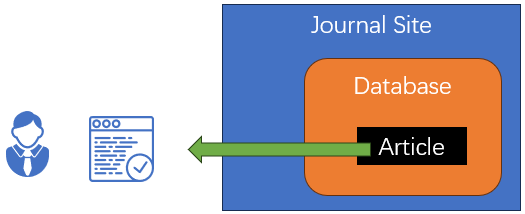
\includegraphics[width=3in]{assets/journalsite.png}
  \label{fig:journalsite}
  \caption{Article in Database}
\end{figure}

When an article is uploaded to a blockchain(Look at Figure \ref{fig:journalchain}), its content, timestamp, and relevant metadata are all recorded on the blockchain. This means that anyone can verify the existence, content, and timestamp of the article. This provides a high level of assurance for the immutability and transparency of documents, particularly with potential significance in research, intellectual property protection, and copyright. Uploading articles to the blockchain also enables decentralized data storage, reducing reliance on centralized institutions. This offers a more open and trustworthy means of data sharing for the academic community and other domains.
%当一篇文章被上链到区块链中,它的内容、时间戳以及相关的元数据都会被记录在区块链上。这意味着任何人都可以验证这篇文章的存在、内容和时间。这为文献的不可篡改性和透明性提供了极高的保障,尤其在科研、知识产权保护和版权方面具有潜在的重要应用。上链文章还可以实现去中心化的数据存储,减少对中央化机构的依赖。这为学术界和其他领域提供了更开放和可信的数据共享方式。

\begin{figure}[h]
  \centering
  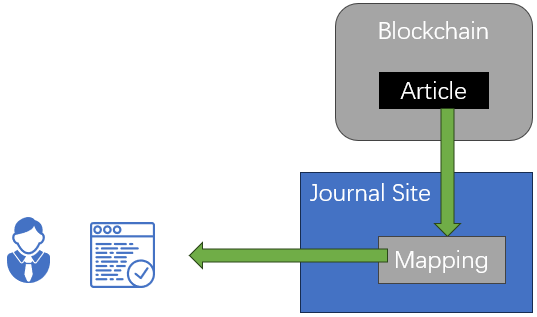
\includegraphics[width=3in]{assets/journalchain.png}
  \label{fig:journalchain}
  \caption{Article in Blockchain}
\end{figure}

Uploading an article to a blockchain, as compared to storing it in a traditional database, provides the author with a clear and objective ownership of the article. In a traditional database, the ownership of the data and the integrity of the database are controlled by the entity or organization managing the database. Authors and other stakeholders may not have direct control or visibility into the ownership and usage of the data.
%将文章上传至区块链,与将其存储在传统数据库中相比,可以让作者更明确且客观地拥有文章。在传统数据库中,数据的所有权和数据库的完整性由管理数据库的实体或组织控制。作者和其他利益相关方可能无法直接控制或了解数据的所有权和使用情况。

On the other hand, when an article is uploaded to a blockchain, the author can have greater confidence in their ownership and control over the article. The blockchain's decentralized and immutable nature ensures that the ownership records are transparent, tamper-resistant, and not under the sole control of a centralized authority. This empowers authors to have a direct and verifiable claim to their work, which can be particularly important for intellectual property protection, copyright, and ensuring that the author's rights are respected.
%另一方面,当文章上传至区块链时,作者可以更有信心地拥有和控制文章。区块链的去中心化和不可篡改性确保了所有权记录的透明性、防篡改性,并不受中心化权威的独立控制。这使作者能够直接并且可验证地主张他们的作品,这对于知识产权保护、版权以及确保作者的权利得到尊重尤为重要。



\textbf{Compared with traditional journals, articles on the chain belong entirely to the author.}
%相比于传统期刊,链上的文章完全属于作者。


\paragraph{Traditional Databases}
%传统数据库:

Traditional databases are typically controlled by a central entity or organization, with database administrators responsible for management and access control. This centralization may result in less transparent ownership.
%传统数据库通常由中央机构或组织控制,数据库管理员负责管理和授予访问权限。这可能导致数据的所有权不够透明。

Access to and modification of data in traditional databases often depend on access controls set by database administrators. This can lead to disputes or lack of transparency regarding data access.
%数据的访问和修改通常依赖于数据库管理员设置的访问控制。这可能导致对数据访问权限的争议或不透明性。

Data in traditional databases can be relatively easily modified or deleted. This may raise concerns about data security and integrity, especially in cases where intellectual property protection is crucial.
%传统数据库中的数据可以相对容易地被修改或删除。这可能引发数据安全性和完整性的问题,尤其是在需要保护知识产权时。

Ownership and control of data are typically centralized with the database administrator. This centralization introduces a single point of control over data usage, increasing the risk of misuse or improper handling.
%数据的所有权和控制通常集中在数据库的管理者手中。这可能导致对数据使用的单一控制点,增加了数据被滥用或不当处理的风险。

\paragraph{Blockchain}
%区块链:

Every transaction on the blockchain has a clear timestamp, documenting the transfer of ownership. This provides authors with a transparent, immutable record of ownership. Authors can trace ownership back to each stage of the data's lifecycle.
%区块链上的每个交易都有明确的时间戳,记录了数据的所有权转移。这为作者提供了清晰、透明且不可篡改的所有权记录。作者可以追溯到每个阶段数据的所有者。

Blockchain utilizes smart contracts to define and enforce data access permissions. This allows dynamic adjustments of data access rights based on different conditions, such as paid access or specific usage licenses.
%区块链可以使用智能合约来定义和执行数据的使用权限。这使得在不同的条件下,如付费访问或特定使用许可下,可以动态地调整数据的访问权限。

Blockchain is decentralized, with data stored across multiple nodes in the network. This ensures that no single central entity can unilaterally control ownership, enhancing data security and tamper resistance.
%区块链是去中心化的,数据存储在网络的多个节点上。这意味着没有单一的中央机构能够单方面控制数据的所有权,增加了数据的安全性和防篡改性。

Once data is written to the blockchain, it is nearly impossible to modify or delete. This ensures the immutability of data, providing robust protection for the author's rights.
% 一旦数据被写入区块链,几乎不可能对其进行修改或删除。这确保了数据的不可篡改性,作者的权利得到了更强有力的保护。

In summary, blockchain offers a more transparent, immutable, and decentralized ownership mechanism, providing stronger protection for authors' intellectual property and data rights. This is particularly advantageous in scenarios where emphasis is placed on data security, traceability, and transparency.using a blockchain for article storage offers authors a more objective and transparent means of claiming ownership of their work compared to traditional database systems.
%综合而言,区块链提供了更为透明、不可篡改、去中心化的拥有权机制,更好地保护了作者的知识产权和数据权益。这对于需要强调数据的安全性、可追溯性和透明性的应用场景非常有利。使用区块链进行文章存储相对于传统数据库系统,为作者提供了更客观和透明的方式来主张他们的作品所有权

\section{Author Finance from Journal}


In the evolution of electronic journals, websites have become the primary medium for disseminating research papers. Although the content of users' papers remains the intellectual property of the authors, the wealth generated by journals through these papers often belongs predominantly to the journals rather than the authors.
%在电子期刊的发展历程中,论文的载体逐渐从传统的印刷版本过渡到了数字化的网站形式。尽管用户的论文内容仍然属于作者的创作成果,然而,由于现行模式下,杂志通过论文创造的财富往往主要归属于杂志自身,而非作者。

In our hypothetical scenario, we contemplate a shift in this paradigm, envisioning a system where a certain proportion of the generated wealth is allocated back to the authors. Taking paid downloads as a simple example, this mechanism aims to provide authors with a more direct economic incentive. Such a transformation not only has the potential to enhance authors' motivation and creativity but also holds the promise of establishing a more equitable wealth distribution system. This envisioned change could contribute to fostering a sustainable and mutually beneficial development model in the realm of electronic journals, addressing the balance of interests between authors and journals more effectively.
% 在当前设想下,我们可以假设一种改进模式,即按照一定比例将创造的财富回馈给作者。以付费下载为例,这一机制可以为作者提供更直接的经济回报。这种变革不仅有助于激发作者的积极性和创作动力,同时也有望促进更公正的财富分配体系的建立。这样的改变有望在电子期刊领域引入更加可持续和互惠的发展模式,从而更好地满足作者和杂志之间的利益平衡。

App that enables users to download papers and make money could be designed:

\begin{enumerate}
  \item {Create a platform: Design an app that provides a platform for users to access academic papers in their field of interest. The app could be designed for both iOS and Android devices.}
  \item {Build a database: Build a database of academic papers from various disciplines that can be downloaded by users. You could partner with universities, libraries, and publishers to acquire the papers.}
  \item {Implement a payment system: Create a payment system that allows users to purchase and download papers. You could charge a fee per paper or offer subscription packages for unlimited access.}
  \item {Integrate social networking features: Incorporate social networking features such as discussion forums, chat rooms, and rating systems to encourage users to engage with the content and with each other.}
  \item {Create an affiliate program: Allow users to earn money by referring other users to the app. You could provide a commission for each new user referred, or offer rewards for reaching certain milestones.}
  \item {Implement security measures: To protect the intellectual property rights of the authors and publishers, implement security measures such as digital rights management (DRM) and watermarking to prevent unauthorized distribution of the papers.}
  \item {Provide customer support: Ensure that users have access to customer support in case they encounter any issues or have questions. }
\end{enumerate}


Overall, designing an app that enables users to download papers and make money requires careful consideration of legal and ethical issues surrounding academic publishing, as well as the needs and preferences of users. It's important to ensure that the app provides value to both users and content creators, while also operating in a fair and ethical manner.

\begin{figure}[h]
  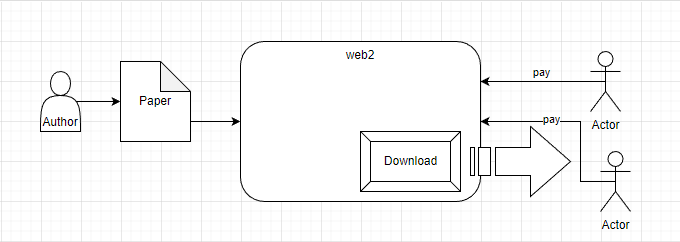
\includegraphics[width=3in]{assets/web2.png}
  \caption{User Pay for Download in Web2.0}
\end{figure}

Web2, also known as the social web, refers to the current state of the internet that we use today, which is primarily focused on social media, e-commerce, and other web-based applications that allow users to interact with each other and with content in various ways. In Web2, payment systems are typically centralized, meaning that they are controlled by a single entity or organization. For example, when we make a purchase on an e-commerce website, we typically use a centralized payment system like PayPal or a credit card. These systems rely on intermediaries to facilitate transactions, which can result in higher transaction fees and longer processing times.

Web3, also known as the decentralized web, represents a shift toward a more open, decentralized, and secure internet that is built on blockchain technology. In Web3, payment systems are decentralized, meaning that they are not controlled by a single entity or organization. Instead, payments are made using cryptocurrency, which is a digital asset that is secured by cryptographic techniques and operates independently of central banks and other financial institutions. Cryptocurrency payments are processed directly between users without the need for intermediaries, which can result in lower transaction fees and faster processing times.

Overall, the main difference in payment systems between Web2 and Web3 is the degree of centralization. Web2 payment systems are centralized, while Web3 payment systems are decentralized. While Web3 is still in its early stages, it has the potential to revolutionize the way we think about payments, transactions, and financial systems.


\begin{figure}[h]
  \centering
  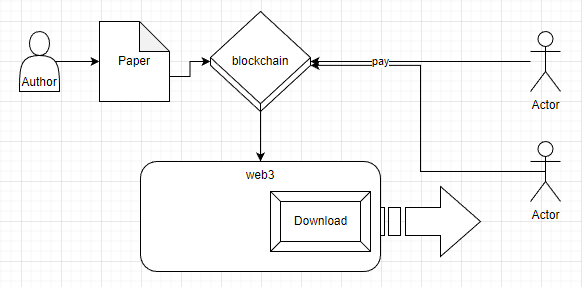
\includegraphics[width=3in]{assets/web3.png}
  \caption{User Pay for Download in Web3.0}
\end{figure}
  

\section{DAO to DeSci}


The DAO, or Decentralized Autonomous Organization, was a decentralized venture capital fund that operated on the Ethereum blockchain in 2016. It was created as a way to enable a group of individuals to pool their resources and invest in new projects without the need for a central authority or intermediary.

The DAO was essentially a smart contract on the Ethereum blockchain that contained a set of rules for how the organization would operate. Members could buy tokens that would give them voting rights to make decisions about which projects to invest in. Once a project was selected, the funds were automatically sent to the project's creators, and the project would be added to the DAO's portfolio.


\begin{figure}[h]
  \centering
  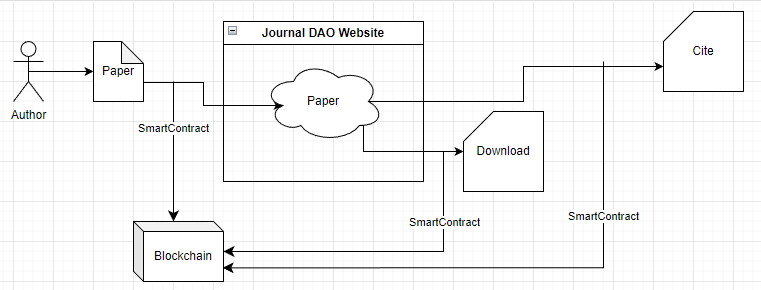
\includegraphics[width=3.2in]{assets/jdao.png}
  \caption{Journal DAO}
\end{figure}

However, the DAO was also susceptible to vulnerabilities, and in June 2016, a hacker exploited a vulnerability in the smart contract, stealing around "\$"50 million worth of Ethereum. This led to a contentious debate within the Ethereum community about how to handle the situation, and ultimately, a hard fork of the Ethereum blockchain was implemented to restore the stolen funds to their original owners.

Despite the controversy surrounding the DAO, it remains an important milestone in the development of blockchain technology, demonstrating the potential of decentralized autonomous organizations to enable new forms of collaboration and investment. Since then, there have been numerous other projects that have built on the DAO's ideas and sought to improve upon its flaws.

Since the DAO incident in 2016, the development of decentralized autonomous organizations (DAOs) has continued to evolve and expand, with new projects and platforms emerging to address the limitations of earlier attempts.

One of the most significant developments in recent years has been the emergence of DAO platforms that offer a more user-friendly and accessible way to create and manage decentralized organizations. These platforms provide tools and templates for creating DAOs, as well as built-in features such as voting, proposal submission, and fund management.

Some of the popular DAO platforms that have emerged in recent years include Aragon, MolochDAO, Colony, and DAOstack. These platforms enable anyone to create and participate in a decentralized organization, with a range of potential use cases such as investment funds, decentralized communities, and decentralized governance.


Another notable development in the DAO space has been the integration of blockchain technology with other emerging technologies, such as non-fungible tokens (NFTs) and decentralized finance (DeFi). For example, some DAOs are exploring the use of NFTs as a way to represent membership or ownership in the organization, while others are using DeFi protocols to manage and distribute funds.

Overall, the development of DAOs continues to evolve and mature, with new ideas and innovations emerging all the time. As blockchain technology and decentralized systems become more mainstream, it is likely that we will see an increasing number of DAOs being created and used for a variety of purposes.


\begin{figure}[h]
  \centering
  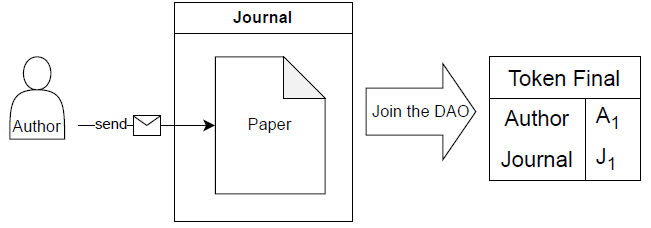
\includegraphics[width=3.2in]{assets/daopaper.png}
  \caption{Distribute Token by DAO}
\end{figure}


After the author publishes the paper in the Web3.0 journal, the paper is stored on a blockchain, afterthen TOKEN is distributed using the DAO framework.


\begin{figure}[h]
  \centering
  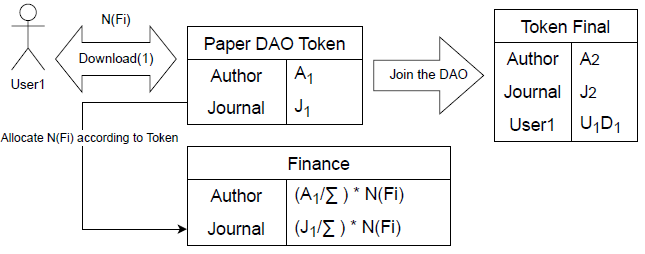
\includegraphics[width=3.2in]{assets/download1.png}
  \caption{Distribute Token while User Download}
\end{figure}


For example, someone downloading papers will creates finance.The funds received will be distributed to all holders in proportion to the token of the DAO framework. After that, users who download the paper will also receive a certain token and will be able to share the funds later. In other words, the user who download thie paper also becomes a holder and also own this paper.


\begin{figure}[h]
  \centering
  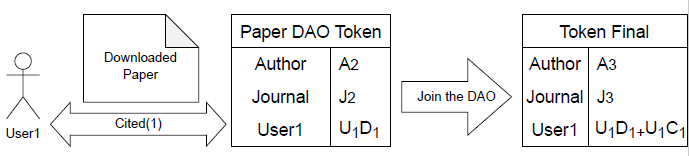
\includegraphics[width=3.2in]{assets/cite1.png}
  \caption{Distribute Token while User Cite Downloaded Paper}
\end{figure}


After downloading the paper, user can cite this paper in own paper and can get more token.


\begin{figure}[h]
  \centering
  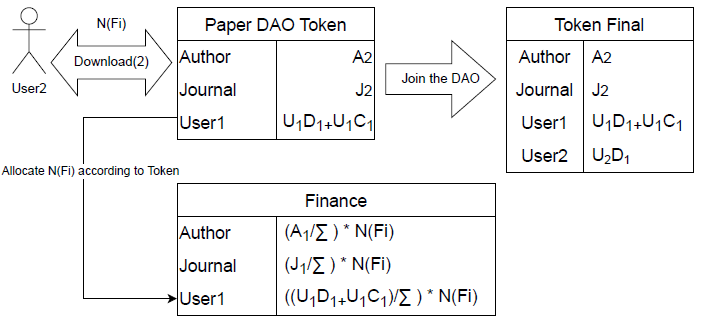
\includegraphics[width=3.2in]{assets/donwload2.png}
  \caption{Distribute Token while Another User Download}
\end{figure}


The currency paid by user2 when downloading the paper will continue to be distributed to all holders in proportion to the token. at this point, the holders already include user1. Both the author and the user who downloaded the paper will own the paper in proportion, and once the paper creates finance, it will be distributed to all owners.

\section{DeFi Deduced}

Defi deduced is a term that could be used to describe the process of applying deductive reasoning to the field of decentralized finance (defi). Deductive reasoning, or deduction, is making an inference based on widely accepted facts or premises. For example, one could deduce that a certain defi protocol is secure if it has been audited by a reputable firm and has no known vulnerabilities. Defi deduced could also refer to the outcome of such reasoning, such as a conclusion or a judgment about a defi project or phenomenon. For instance, one could deduce that the demand for defi services is increasing if the total value locked (TVL) in defi platforms is rising. Defi deduced could be seen as a way of applying logic and rigor to the analysis and evaluation of defi, which is a complex and dynamic domain that involves various aspects such as cryptography, economics, governance, and social behavior.


\section{Conclusion}


DAOs have several advantages over traditional organizations, such as:

\begin{itemize}
\item{Lower costs: DAOs eliminate the need for intermediaries, lawyers, accountants, or managers, reducing the overhead and bureaucracy involved in running an organization.}
\item{Higher efficiency: DAOs enable faster and more accurate decision-making, as well as automated execution of tasks and transactions.}
\item{Greater innovation: DAOs foster a culture of experimentation and creativity, as anyone can propose and contribute to new ideas or initiatives.}
\item{Enhanced security: DAOs are protected by cryptography and consensus mechanisms, making them immune to hacking, fraud, or manipulation.}
\item{Increased inclusivity: DAOs are open and accessible to anyone who shares the vision and values of the organization, regardless of their location, background, or status.}
\end{itemize}

DAOs are not without challenges, however. Some of the main challenges include:

\begin{itemize}
\item{Legal uncertainty: DAOs operate in a gray area of the law, as they do not fit into existing legal frameworks or jurisdictions. This creates risks and liabilities for the participants and the beneficiaries of the DAO.}
\item{Ethical dilemmas: DAOs may face ethical issues or conflicts of interest, as they may not align with the moral values or social norms of the wider society.}
\item{Technical complexity: DAOs rely on complex and experimental technologies, such as blockchain and smart contracts, which may have bugs, vulnerabilities, or unforeseen consequences.}
\item{Governance issues: DAOs may struggle to achieve consensus, resolve disputes, or adapt to changing circumstances, as they lack a clear leadership or authority structure.}
\end{itemize}


% \section*{Acknowledgments}
% This should be a simple paragraph before the References to thank those individuals and institutions who have supported your work on this article.



% {\appendix[Proof of the Zonklar Equations]
% Use $\backslash${\tt{appendix}} if you have a single appendix:
% Do not use $\backslash${\tt{section}} anymore after $\backslash${\tt{appendix}}, only $\backslash${\tt{section*}}.
% If you have multiple appendixes use $\backslash${\tt{appendices}} then use $\backslash${\tt{section}} to start each appendix.
% You must declare a $\backslash${\tt{section}} before using any $\backslash${\tt{subsection}} or using $\backslash${\tt{label}} ($\backslash${\tt{appendices}} by itself
%  starts a section numbered zero.)}



%{\appendices
%\section*{Proof of the First Zonklar Equation}
%Appendix one text goes here.
% You can choose not to have a title for an appendix if you want by leaving the argument blank
%\section*{Proof of the Second Zonklar Equation}
%Appendix two text goes here.}




\bibliography{refs}
\bibliographystyle{IEEEtran}


\newpage

\section{Biography Section}
If you have an EPS/PDF photo (graphicx package needed), extra braces are
 needed around the contents of the optional argument to biography to prevent
 the LaTeX parser from getting confused when it sees the complicated
 $\backslash${\tt{includegraphics}} command within an optional argument. (You can create
 your own custom macro containing the $\backslash${\tt{includegraphics}} command to make things
 simpler here.)
 
\vspace{11pt}

\bf{If you include a photo:}\vspace{-33pt}
\begin{IEEEbiography}[{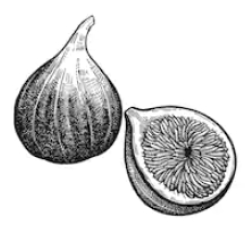
\includegraphics[width=1in,height=1.25in,clip,keepaspectratio]{fig1}}]{Michael Shell}
Use $\backslash${\tt{begin\{IEEEbiography\}}} and then for the 1st argument use $\backslash${\tt{includegraphics}} to declare and link the author photo.
Use the author name as the 3rd argument followed by the biography text.
\end{IEEEbiography}

\vspace{11pt}

\bf{If you will not include a photo:}\vspace{-33pt}
\begin{IEEEbiographynophoto}{John Doe}
Use $\backslash${\tt{begin\{IEEEbiographynophoto\}}} and the author name as the argument followed by the biography text.
\end{IEEEbiographynophoto}




\vfill

\end{document}


